\subsection{POC 2: Auto-Complete for Conference Registration in Indico}

The second prototype aims at connecting Solid with the conference registration module in Indico. When registering for a conference an \gls{html} form is presented with fields previously defined by the conference manager, who deemed those fields necessary. A form always contains personal information of name and email address, but is not limited to it and can even range to more sensible information such as copies of personal identification documents. Information of this type has perfect motivation to remain in the hand of the owner and not be stored in a remote data store, uncontrollable and unknown to the registrants.

Therefore, the aim is to extend the registration module to allow storage in a data pod, where the user has full control and can handle the data to their own liking.

\subsubsection{Architectural Analysis and Synthesis}\mbox{}\\

\paragraph{System Description}\mbox{}\\
\paragraph{Features}\mbox{}\\
\paragraph{Context Diagram}\mbox{}\\
\paragraph{Sequence Diagram}\mbox{}\\

\begin{figure}[H]
    \centering
    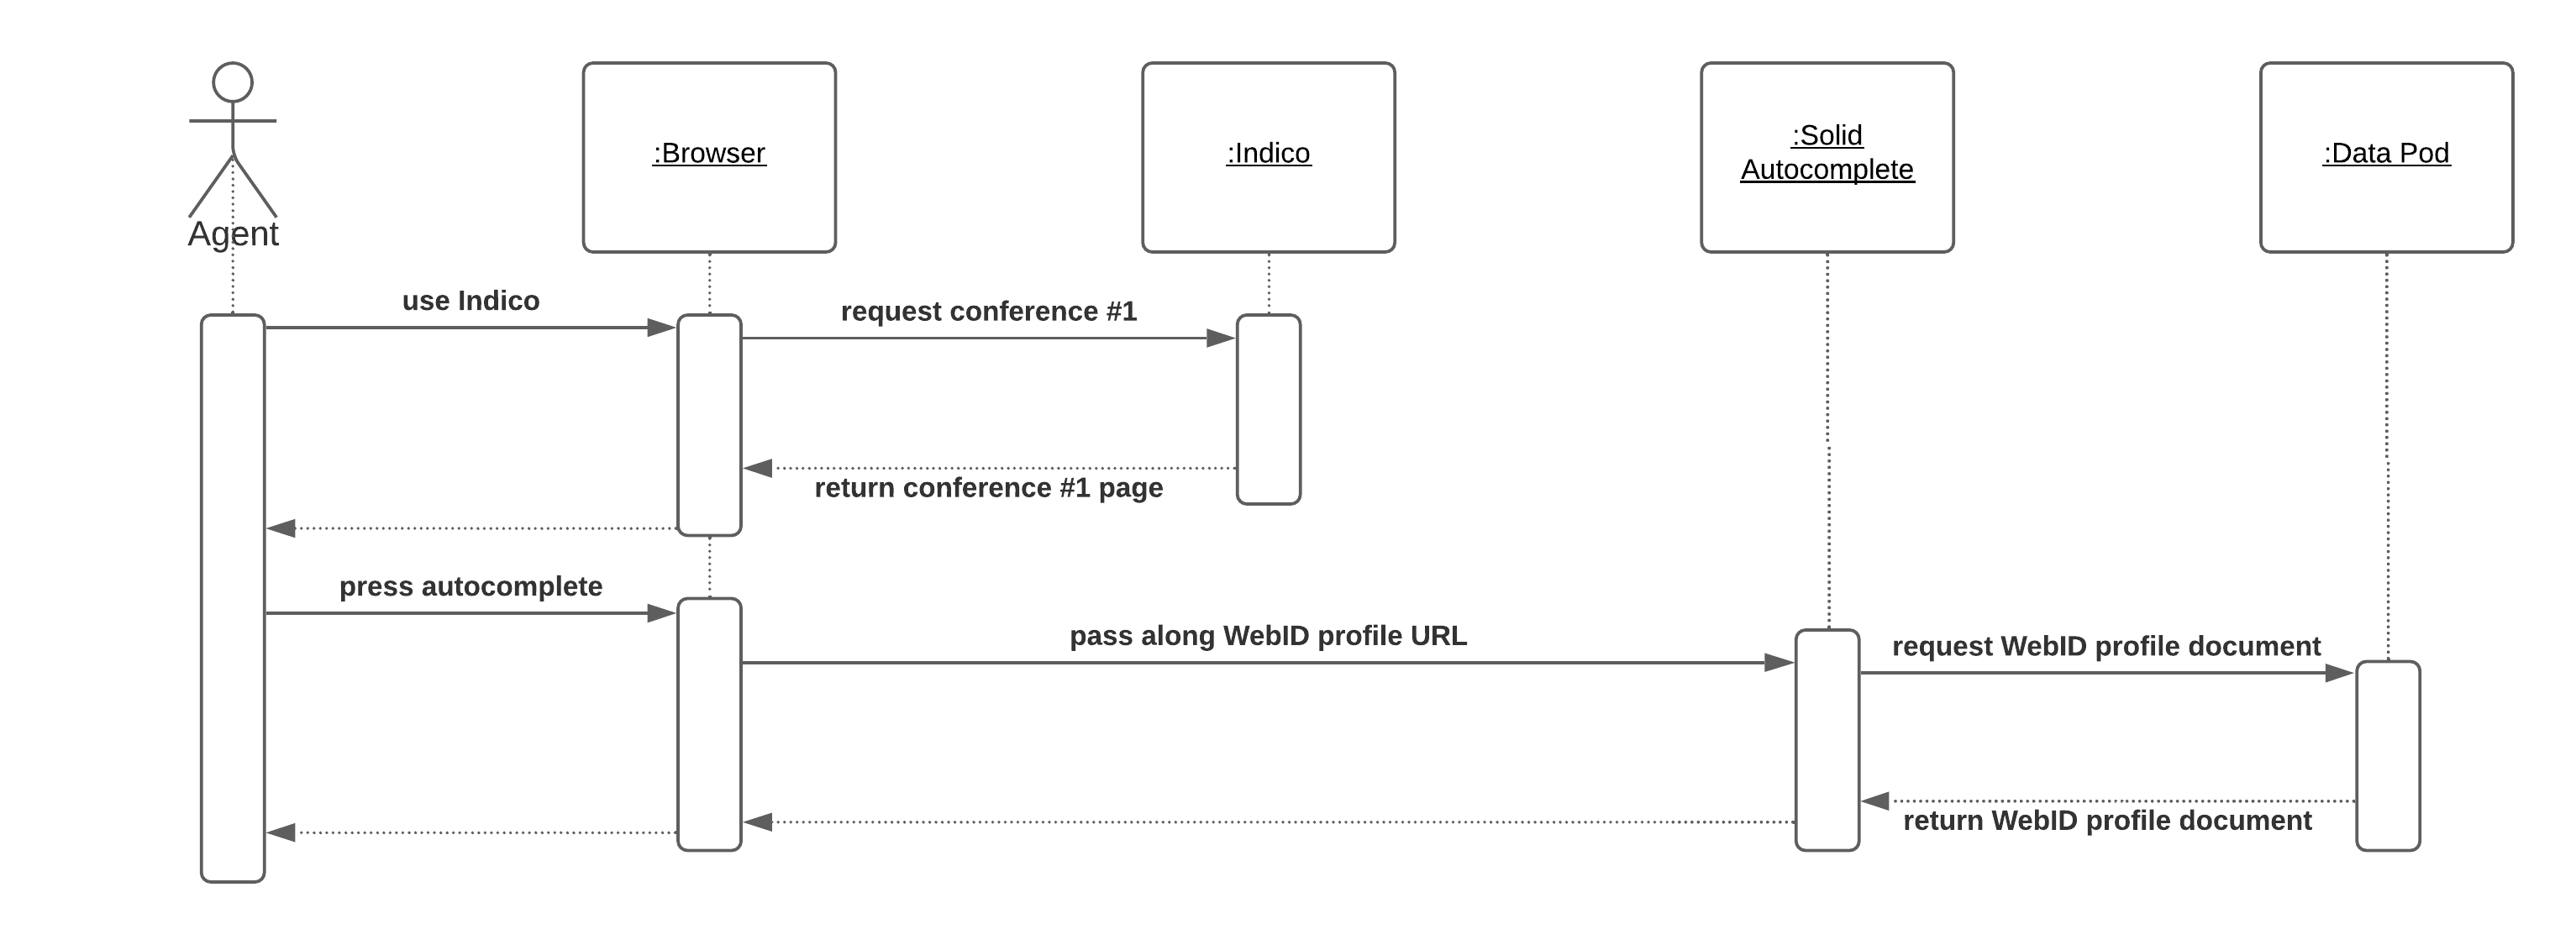
\includegraphics[width=\textwidth]{prototype/graphs/poc-conference_registration-autocomplete-sequence_diagram.png}
    \caption{Sequence diagram showing the sequential process through posting a comment.}
    \label{fig:poc-conference_registration-autocomplete-sequence_diagram}
\end{figure}

\paragraph{Stakeholders}\mbox{}\\
\paragraph{Drivers}\mbox{}\\

\subsubsection{Design}\mbox{}\\

TODO:
1st iteration, save data in pod
2nd iteration, only pull data from pod

TODO: Include these somehow:

\begin{figure}
    \centering
    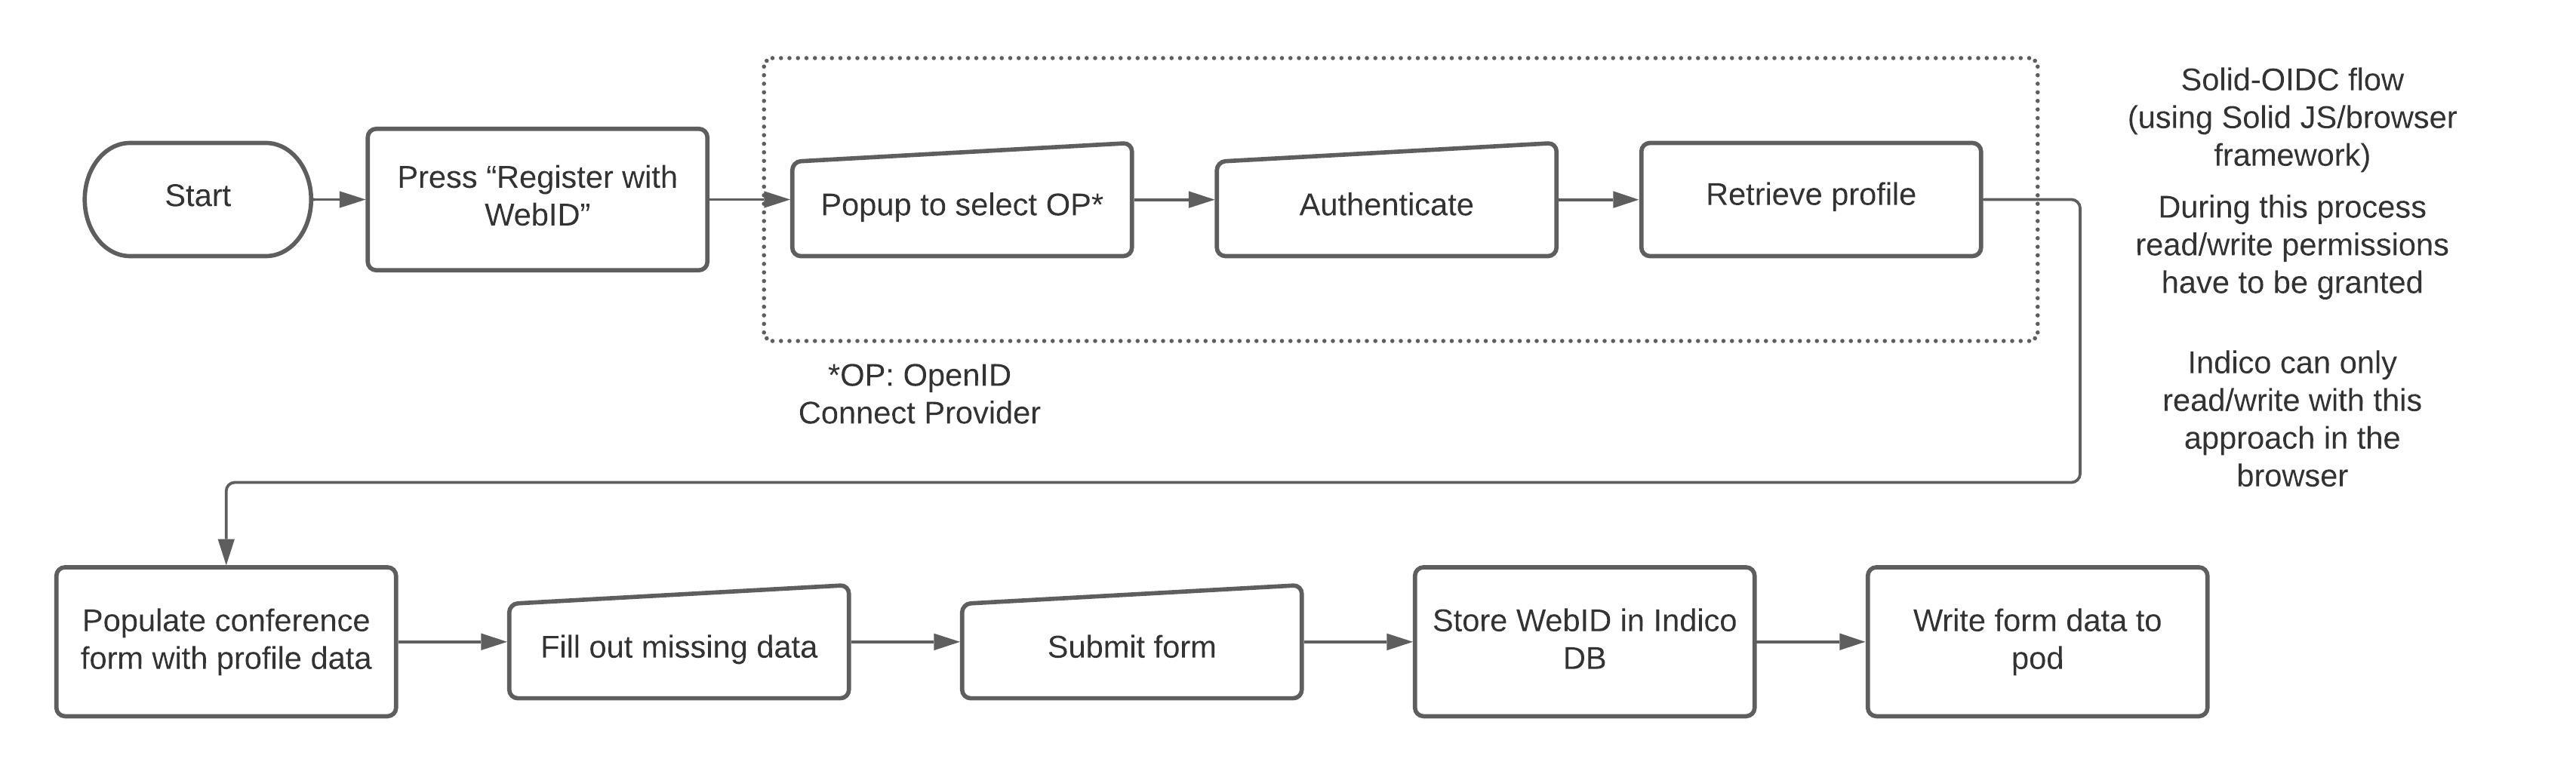
\includegraphics[width=0.6\textwidth]{prototype/graphs/poc-conference_registration_flow-client_side-sideways.jpeg}
    \caption{TODO:}
    \label{fig:poc-conference_registration_flow-client_side-sideways}
\end{figure}

\begin{figure}
    \centering
    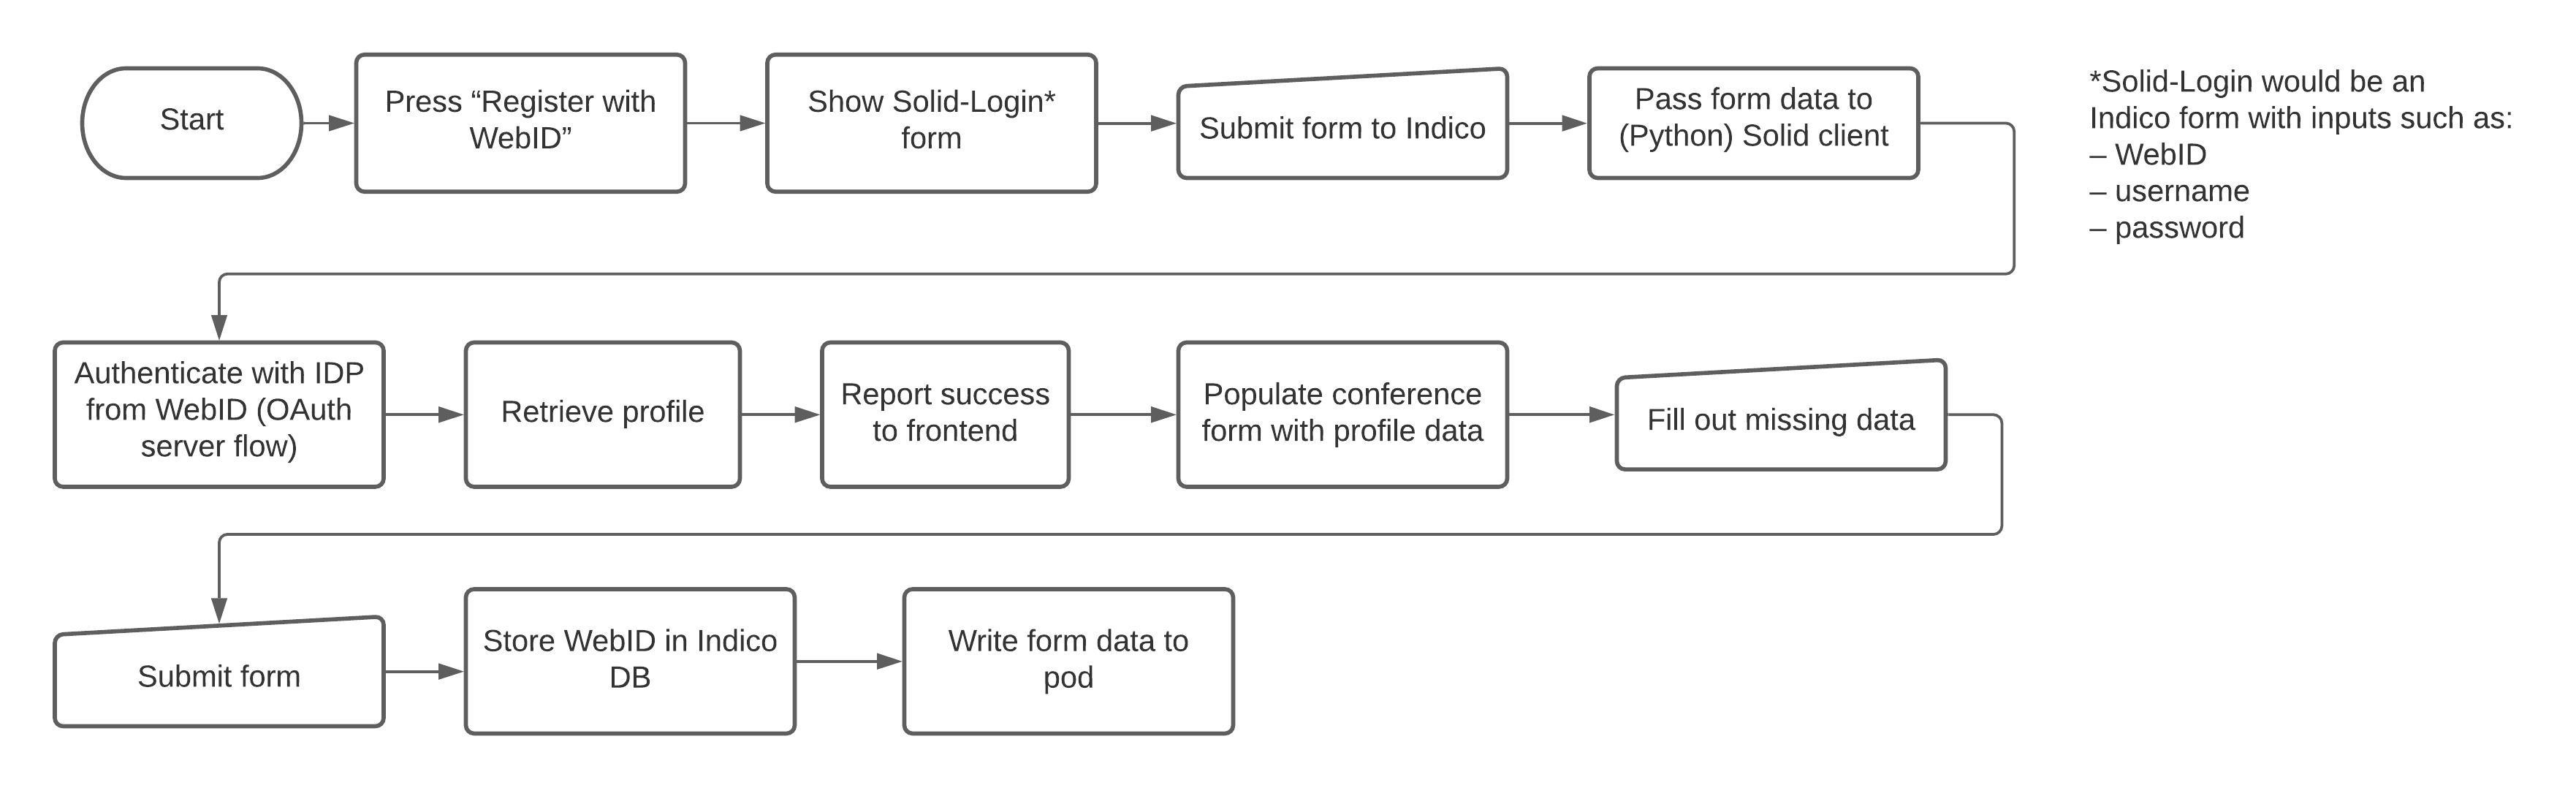
\includegraphics[width=0.6\textwidth]{prototype/graphs/poc-conference_registration_flow-server_side-sideways.jpeg}
    \caption{TODO:}
    \label{fig:poc-conference_registration_flow-server_side-sideways}
\end{figure}

\begin{figure}
    \centering
    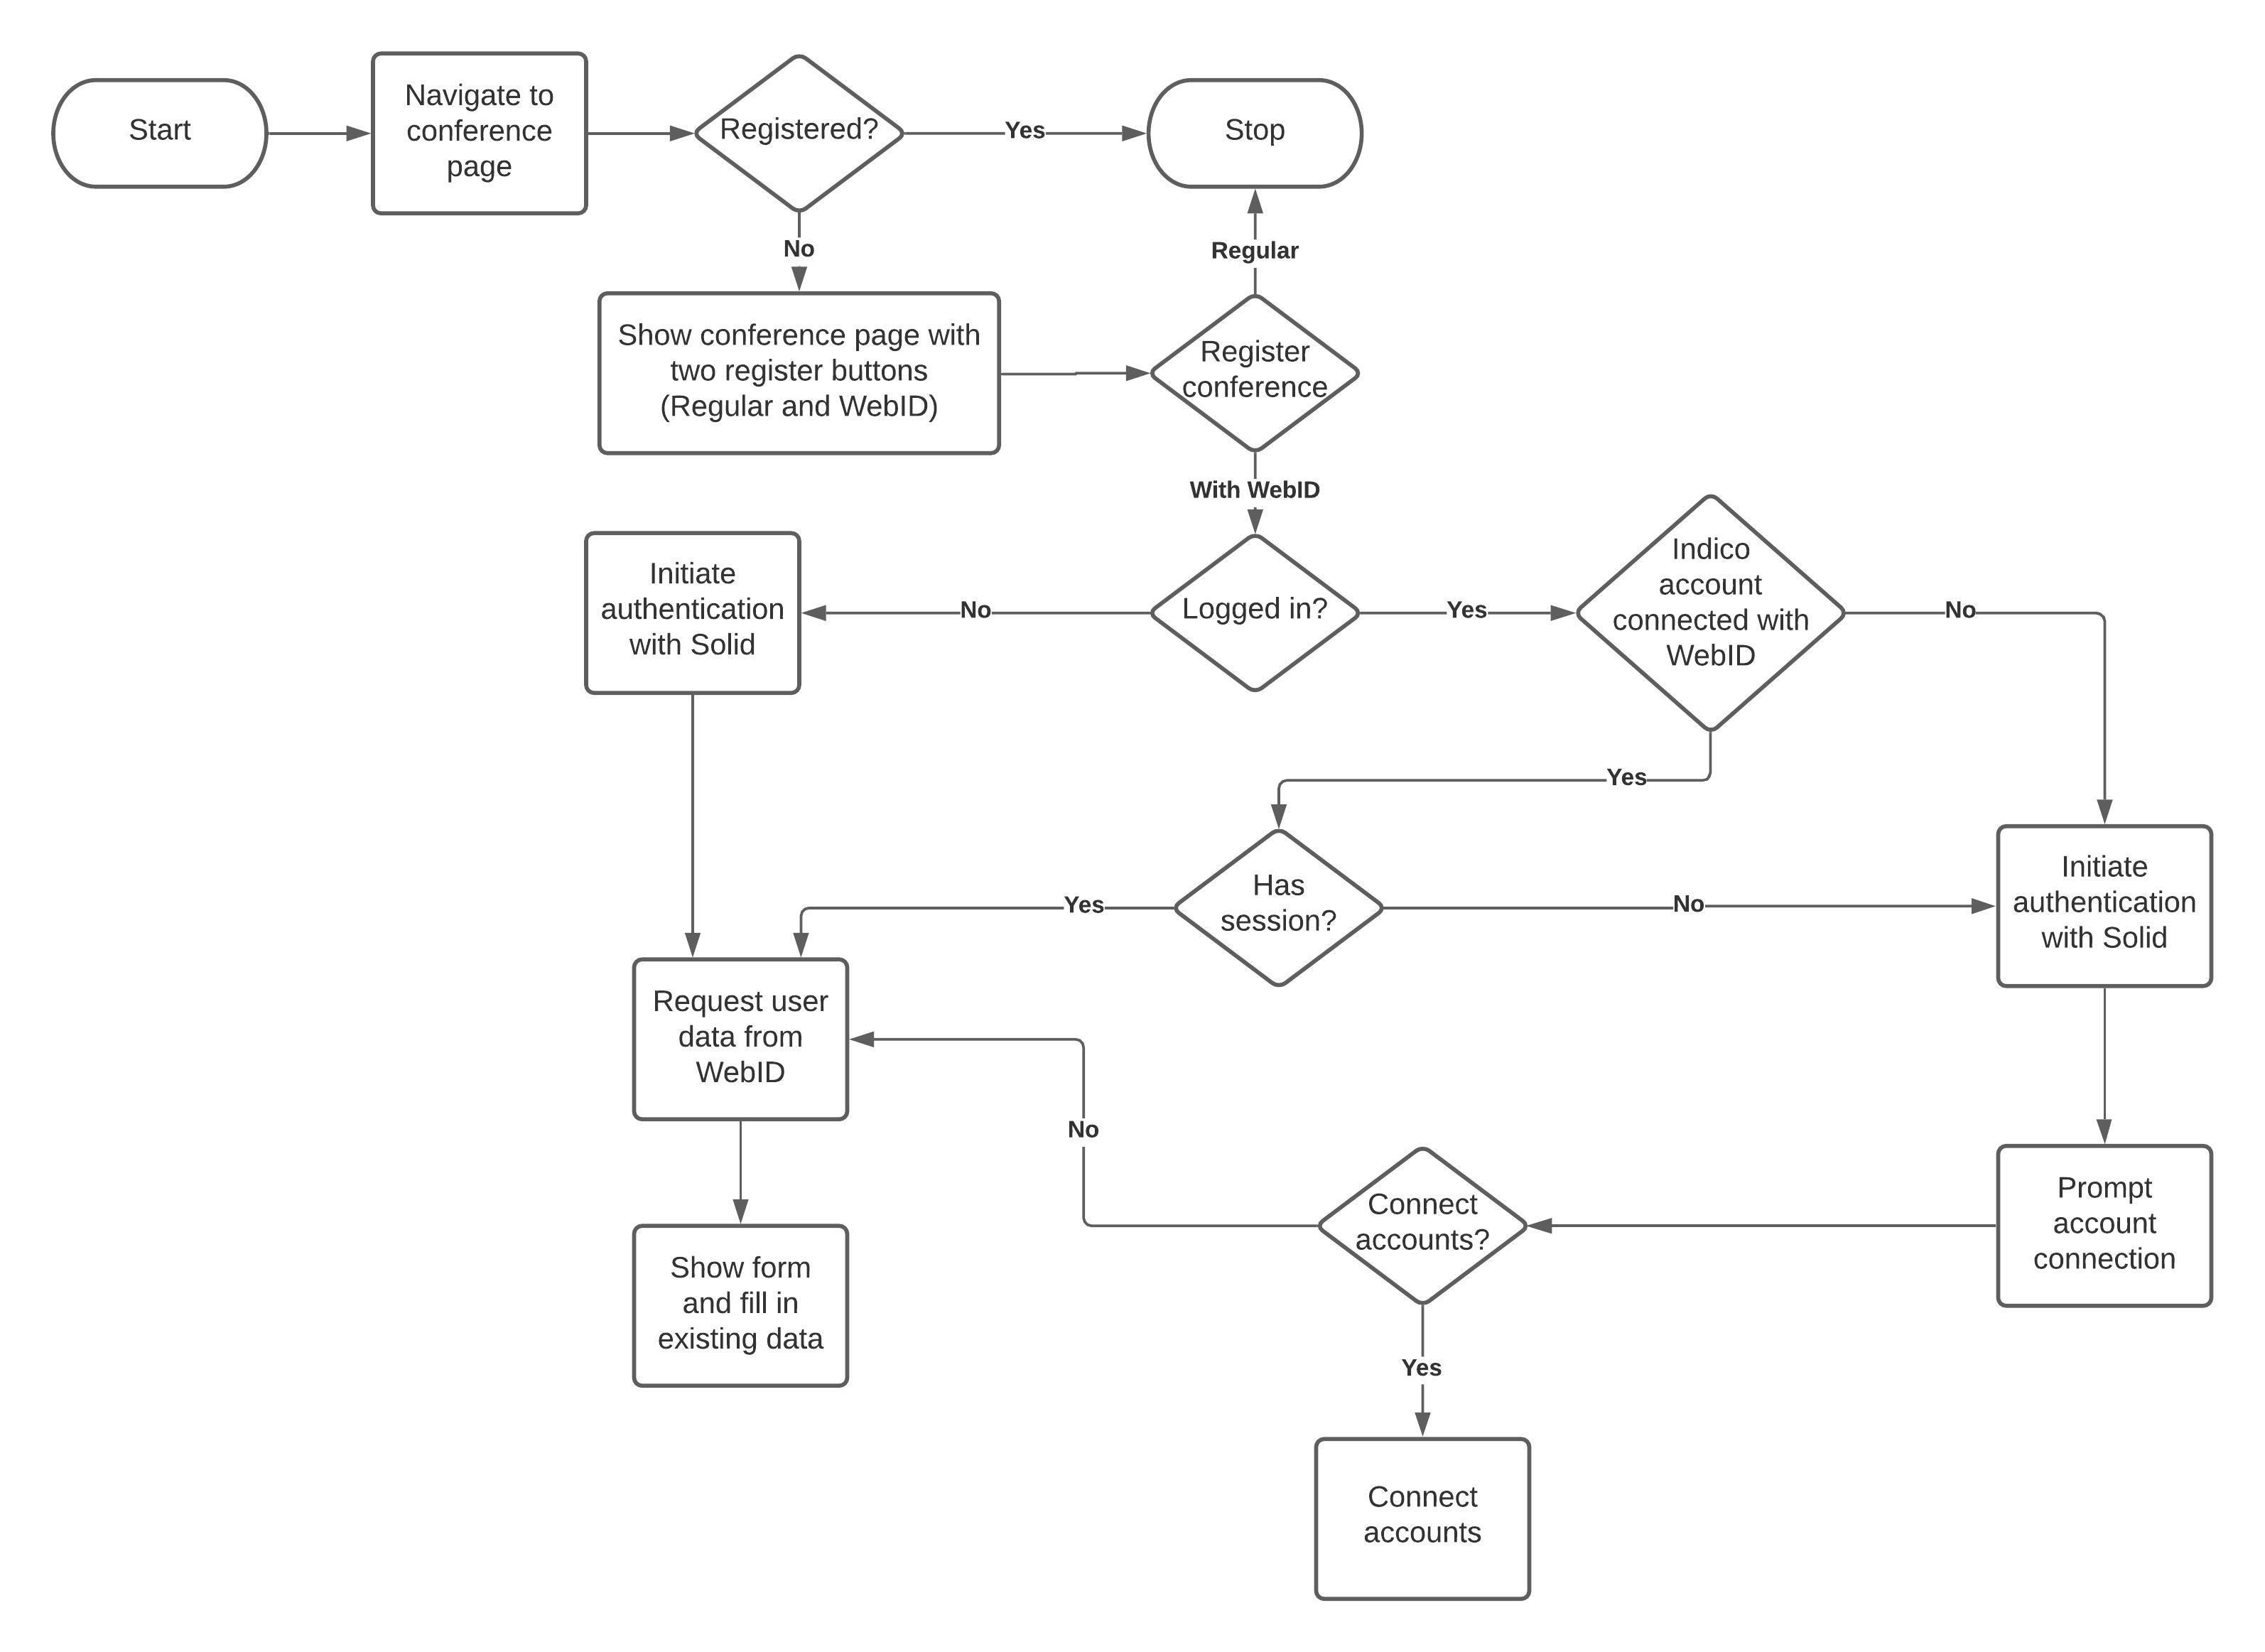
\includegraphics[width=0.6\textwidth]{prototype/graphs/poc-conference_registration_flow-sideways.jpeg}
    \caption{TODO:}
    \label{fig:poc-conference_registration_flow-sideways}
\end{figure}

* Gave up usage control
  * Why it didn't work, and **what is necessary to make it work**
    * usage control
    * question the choice of Indico usage control
    * versioning of tag of personal data
* high-level constraints
* implementation
  * indico limits this
* if indico in this way or more generally

\paragraph{Modification of Resource From Data Pod}\mbox{}\\

\paragraph{Payment on Input Fields}\mbox{}\\

\paragraph{Performance of Large Conference}\mbox{}\\

\paragraph{Availability of Crucial User Data}\mbox{}\\

\subsubsection{Integration With Indico}\mbox{}\\

\paragraph{Bind to Dynamically Created Form}\mbox{}\\

Indico builds the registration form dynamically using a frontend library called AngularJS \cite{angularjs}. This introduces a challenge of interacting with the form using \gls{js}. Frontend libraries that either create new or modify existing \gls{dom} nodes need to wait until the complete \gls{dom} tree is loaded, as they bind to one \gls{dom} node from the initially served \gls{html} document and then do their operations on this node. Meaning, AngularJS waits until the whole \gls{html} document is parsed and rendered in the browser and then starts creating its form from scratch, which is then being rendered by the browser. The problem with this is in order to operate on the form, which is necessary for the module to be able to read the form inputs and labels and also to set their values, the \gls{js} code from this prototype needs to know when the form was successfully rendered. Three options are possible to achieve this.

\begin{enumerate}
    \item Implement the autocomplete functionality in the existing AngularJS form code
    \item Dispatch an event to notify the autocomplete module the form has been rendered
    \item Use the \texttt{MutationObserver} to detect the form creation
\end{enumerate}

Solutions 1 and 2 both involve the need to work with the AngularJS form, which is written in a legacy version and was recommended by an Indico developer to -- if possible -- be avoided. Indico developers also plan on removing AngularJS all together and replace it by a more popular frontend framework. Therefore, option 3 was chosen even though the usage of a \texttt{MutationObserver} instance might add performance degradation to the page load \cite{dom-spec}. The performance shall not be analyzed more carefully as it is not of relevance to proof the realization of the prototype.

The \texttt{MutationObserver} is initialized as soon as the \gls{dom} is rendered, it then takes a node as a target to observe and will register all modifications on this node: creation of children nodes in it, updates to the node itself or any other modifications. To reduce computation the Indico code can be analyzed to find a suitable \gls{dom} element to have as a target node. This node needs to exist when the \gls{dom} is loaded and needs to contain the final form node. When looking at final rendered document containing the AngularJS form one notices that the form has an ID, which can be used to observe its creation.
 
\begin{lstlisting}[language=Other,columns=fullflexible, caption={Observe function in Indico}, label={lst:indico-observe}]
function observeFormCreation() {
  // ID of the AngularJS form, its creation needs to be observed
  const formId = 'registrationForm';
  // Candidate to limit observing scope
  const $conferencePage = document.querySelector('.conference-page');
  const targetNode = $conferencePage;
  // Only observe nodes, not attributes
  const config = {attributes: false, childList: true, subtree: true};

  const callback = (mutationsList, observer) => {
    // Contains all mutations in the targetNode
    for (const mutation of mutationsList) {
      // Node has beed added or removed
      if (mutation.type === 'childList') {
        // Look at all added nodes
        for (const node of mutation.addedNodes) {
          // Look for the AngularJS form
          if (node.id === formId) {
            // Once found, stop observing
            observer.disconnect();
            // Initialize the autocomplete library
            const solidAutocomplete = new SolidAutocomplete({form: node});
            solidAutocomplete.createAutocompleteDomControls(node);
          }
        }
      }
    }
  };
  // Start observing
  const observer = new MutationObserver(callback);
  observer.observe(targetNode, config)
}
\end{lstlisting}
 
\subsubsection{Evaluation}\mbox{}\\

\paragraph{Metrics}\mbox{}\\
\paragraph{Levels}\mbox{}\\
\paragraph{Components}\mbox{}\\

\subsubsection{Analysis}\mbox{}\\

* performance?
* Management part of Indico
  * Forward data between people
  * **Also serve data to people (admin of registration)**
* Comments are more clear tied to comment

* the flow of Solid (ref Tim from White Area) notifying for future conference